\subsection{Energetics}
\textbf{(i, ii)} The total energy, kinetic energy and potential energy can be seen in \autoref{fig:energy}. The change in energy ratio can also be seen. The theoretical values for the finite domain ($\int_{Lx/2}^{Lx/2}$) are also included. One can clearly see that the smallest rossby radius agrees well with the theoretical derived energy loss and ratios. For the larger rossby radii, a larger discrepancy can be seen. Firstly, one can see that the total energy is lower then the theoretically expected total energy for the larger radii. One can observe that this loss is seen in both the potential and kinetic energy, which makes sense since these are a coupled system. However, by viewing the energy ratio, the largest difference is seen in the kinetic energy. 

The reason for the extra energy loss cannot be explained by Poincaré only, since this would only stand for one third of the energy loss. The largest energy loss can be attributed to the small domain size for the larger Rossby radii. Since the domain cannot capture the entire free surface solution $\eta(x,t\rightarrow\infty)$, the potential energy decreases. Since this is coupled to the meridional velocity, the kinetic energy will also decrease. Energy loss can also be attributed to the sponge 'eating energy', and small scale dissipation. 

\begin{figure}[H]
    \centering    
    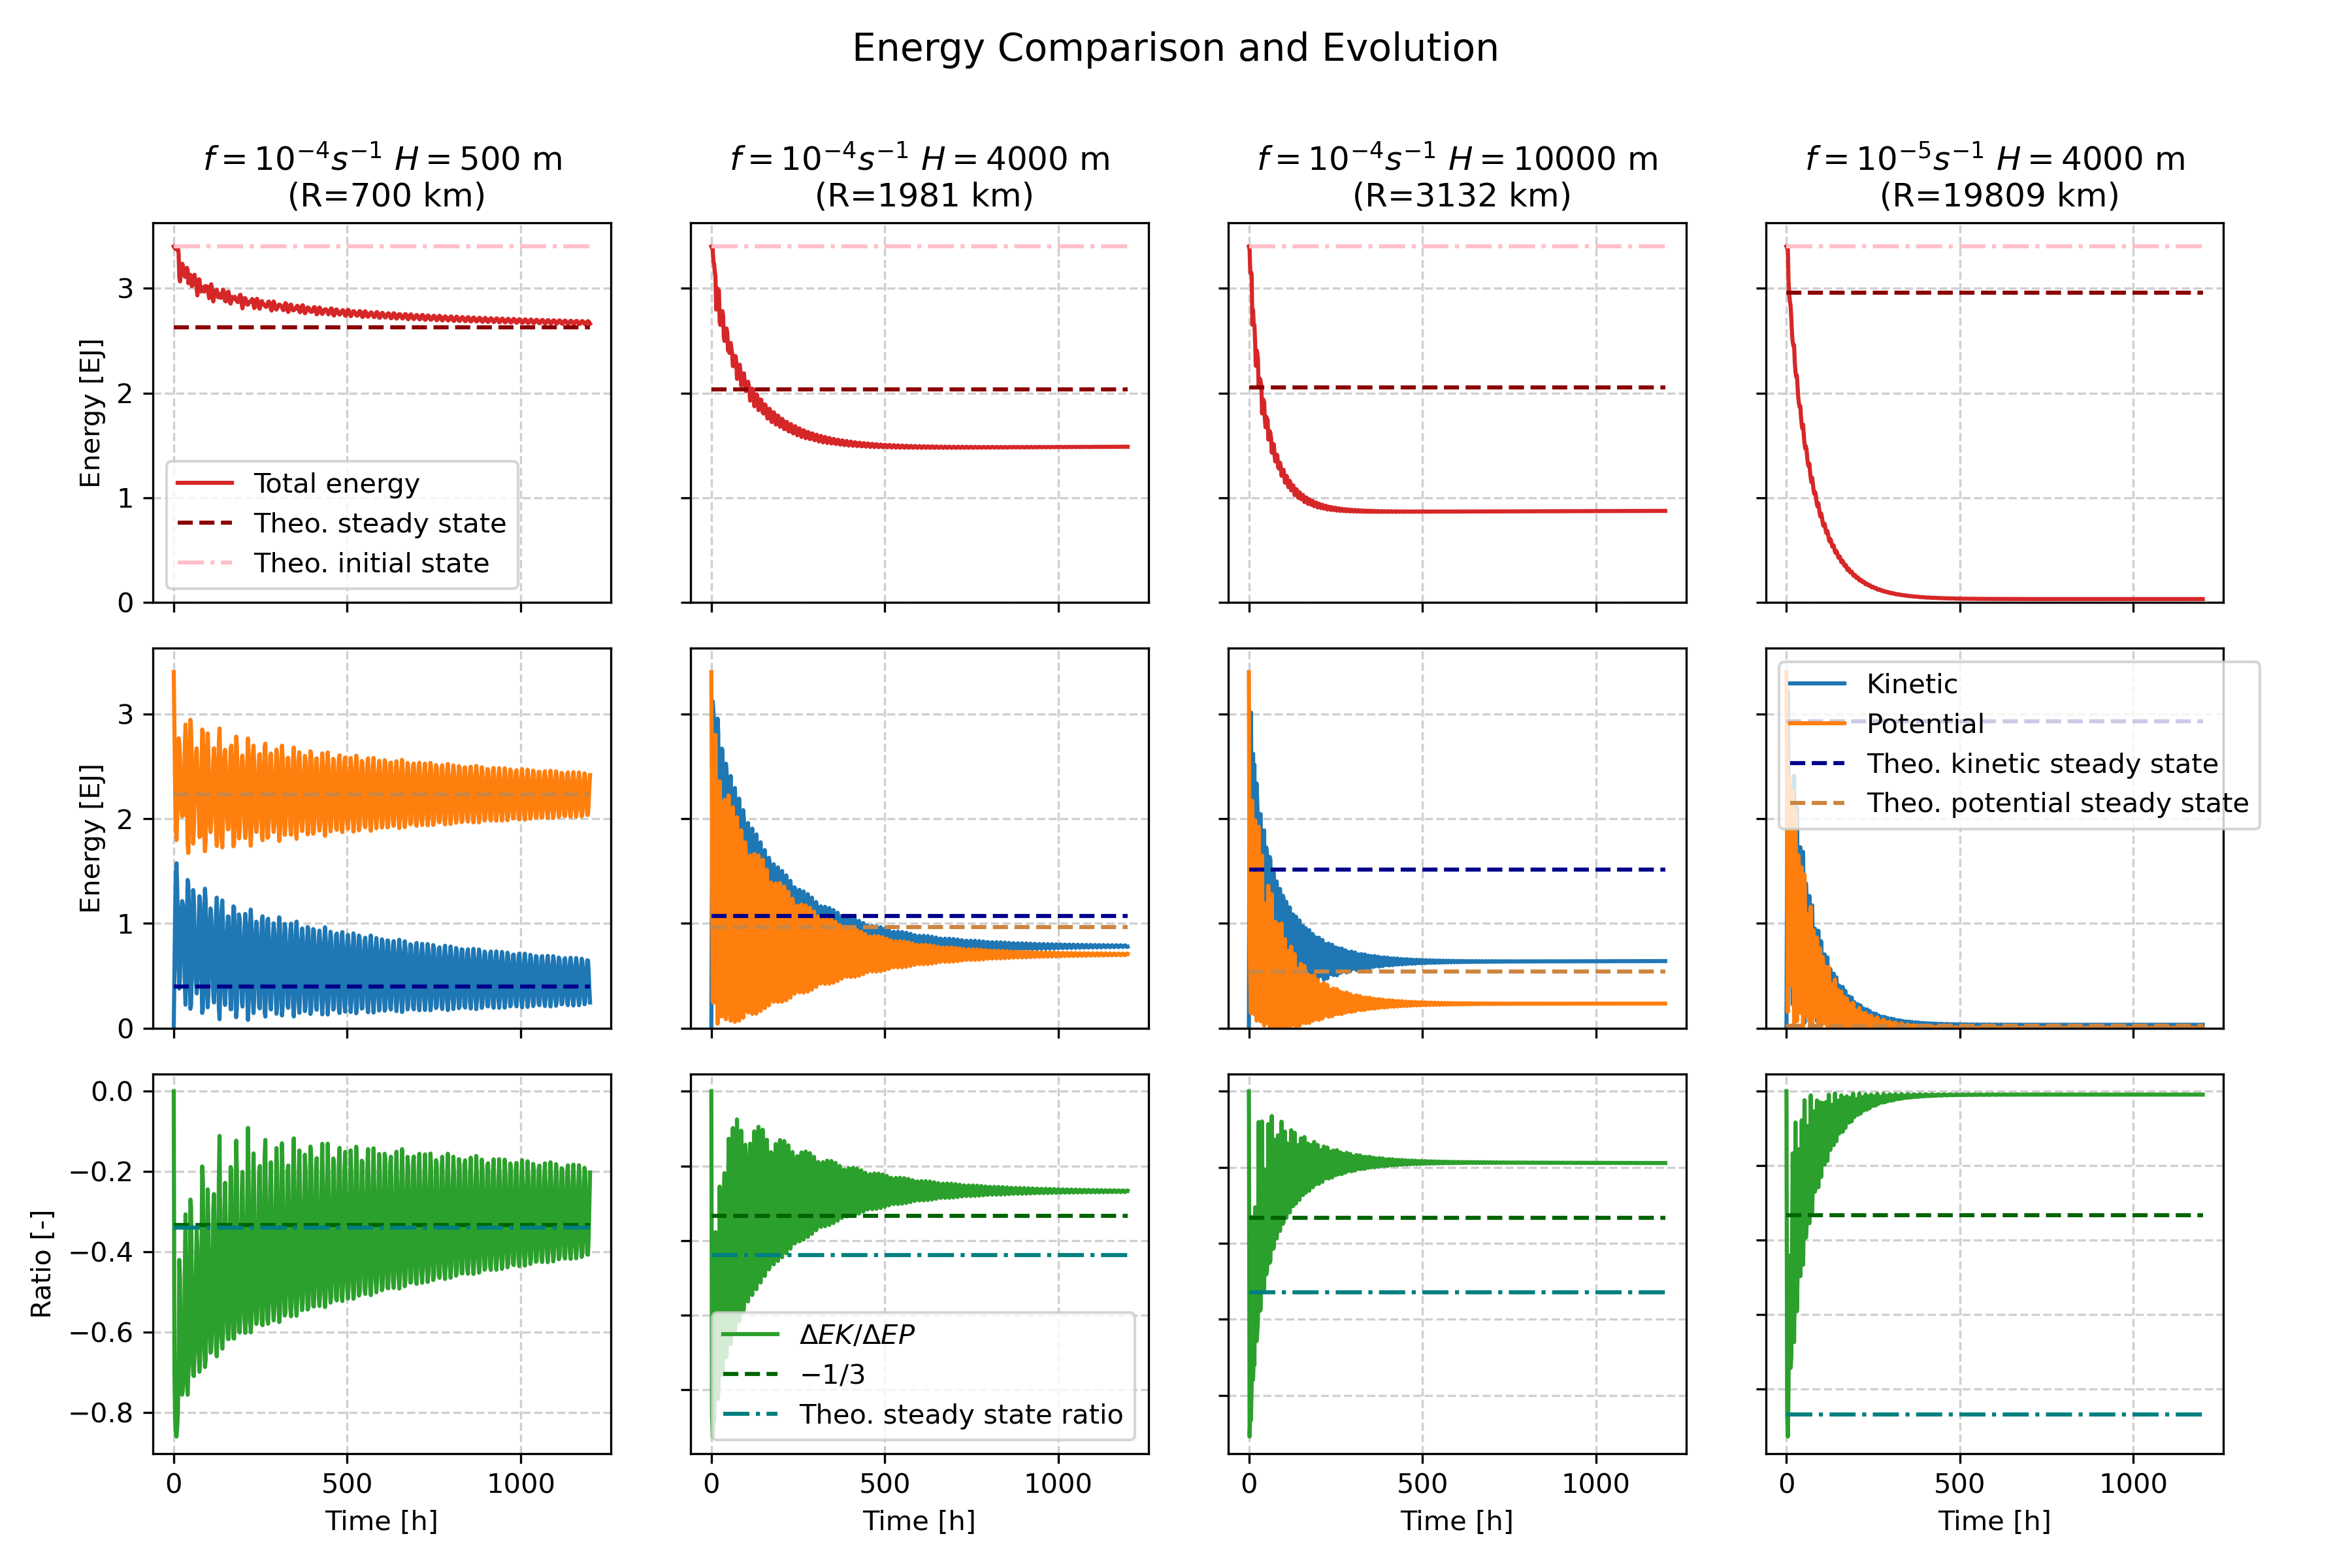
\includegraphics[width=0.9\textwidth]{Figures/energy_comparison.png}
    \caption{This figure shows the energy for the different Rossby radii. Note that the theoretical steady state solutions was plotted using the finite domain, and not the infinite domain.}
    \label{fig:energy}
\end{figure}

Increasing the domain size to $12000$ km $\times$ $9000$ km, for the case when $R=1981$km, can be seen in \autoref{fig:energy_large}. Here we can see that the domain size is now able to capture the entire solution $\eta(x,t\rightarrow\infty)$. ALso, the energy loss is as expected from the theoretical calculation. The energy ratio is also much better then before. This shows that the domain size was indeed a very limiting factor for the larger Rossby radii.  

\begin{figure}[H]
    \centering    
    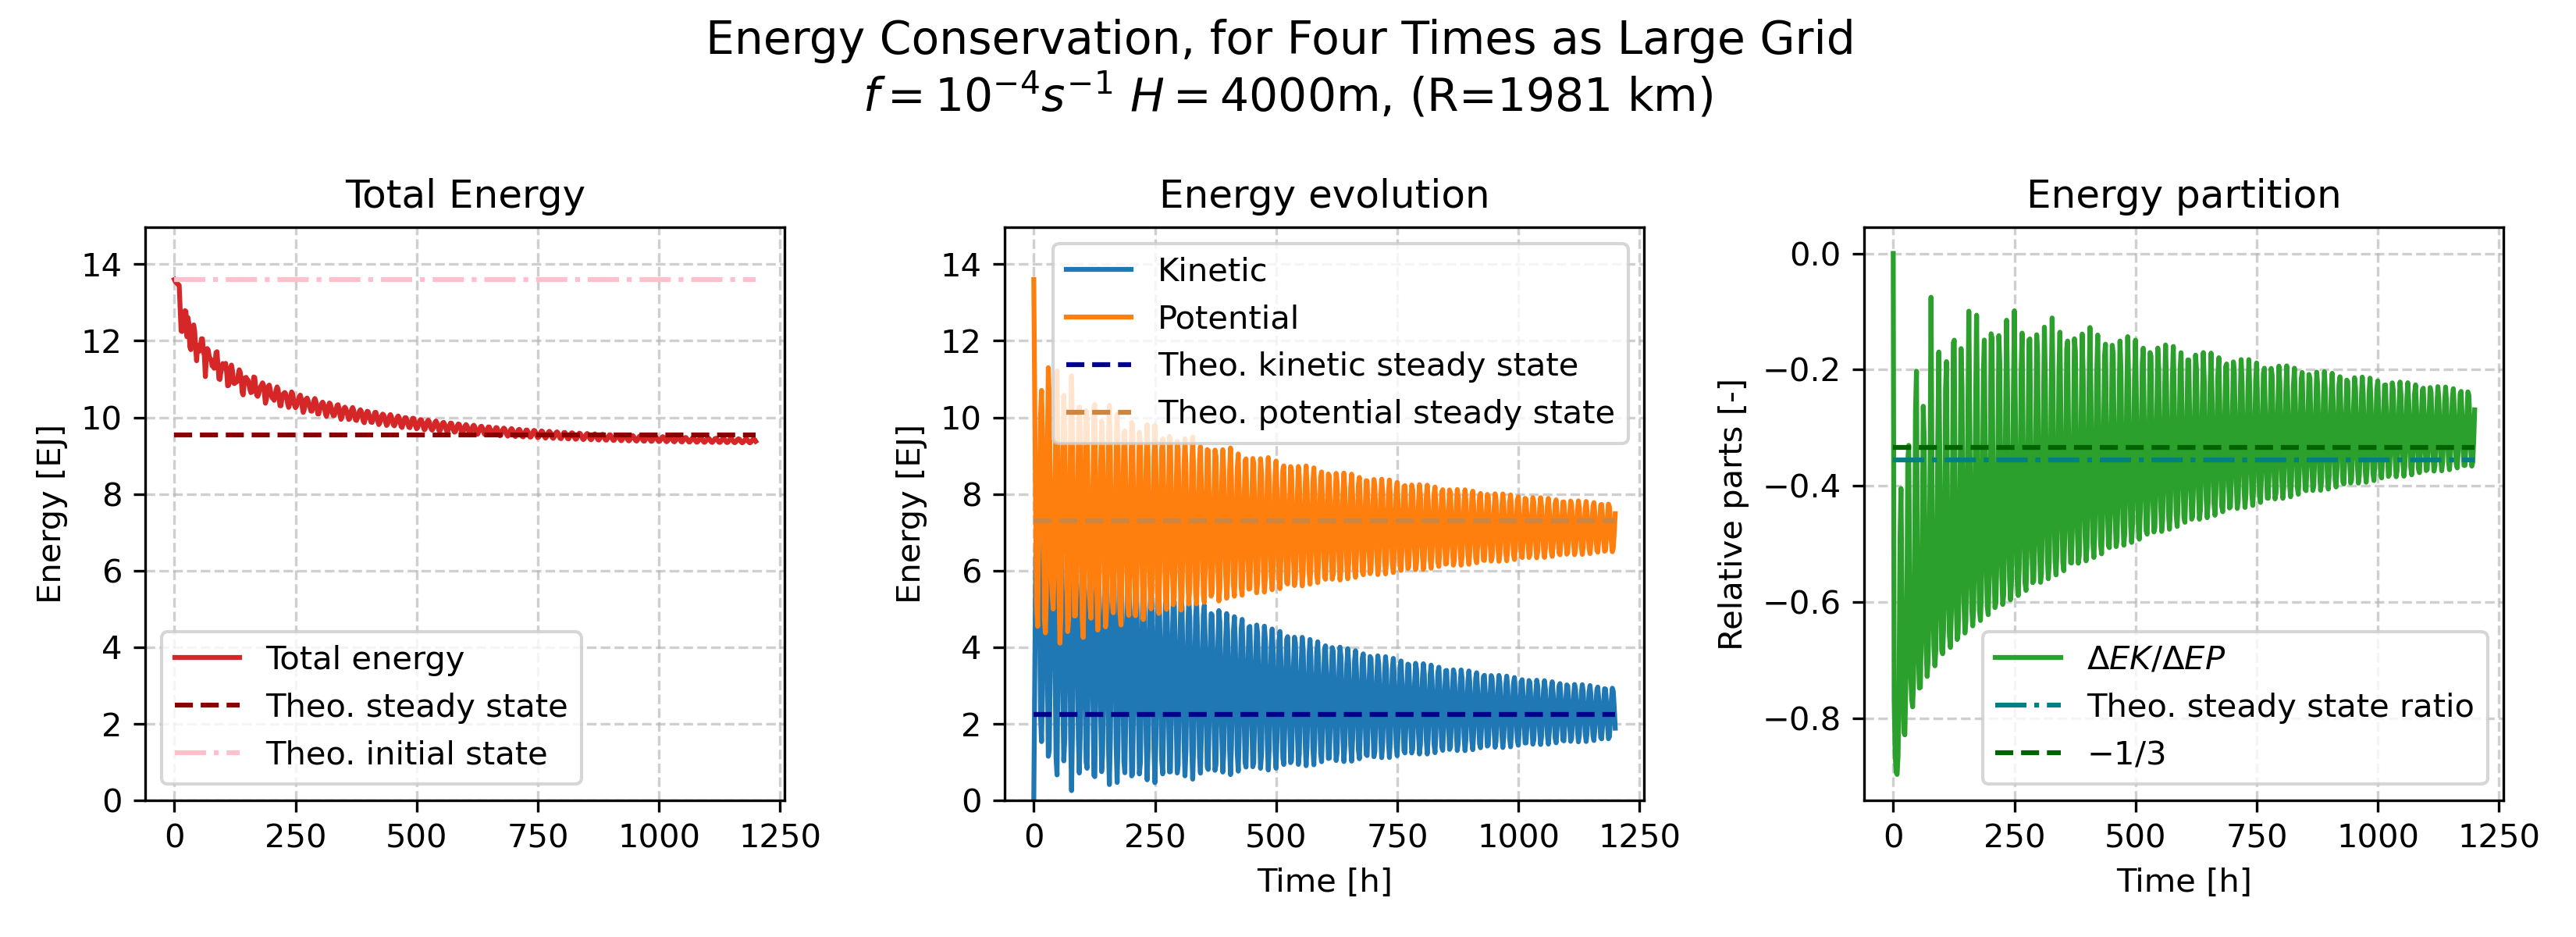
\includegraphics[width=0.7\textwidth]{Figures/energy.png}
    \caption{This figure shows the energy for when the grid size is increased to $12000$ km $\times$ $9000$ km. Note that the theoretical steady state solutions was plotted using the finite domain, and not the infinite domain. The domain size is $6000$ km $\times$ $4500$ km.}
    \label{fig:energy_large}
\end{figure}


\textbf{(iii)} When the domain size is of the right size to capture the Rossby radius ( i.e. $R<Lx,Ly$), then the numerical model agrees well with the theoretical model. One could see that a third of the energy was lost from the initial energy in the system. This can be attributed to the Poincaré waves, moving away with the energy. The remaining energy was split between the potential and kinetic energy, as explained by the theory. There is always a little bit of less potential energy then expected, which can be attributed to the asymptotic nature of the free surface solution $\eta(x,t\rightarrow\infty)$ (see \autoref{eq:solh}). Thus, in reality one would always need an infinite domain to capture the entire solution, but when $L_x>R$ we come pretty close. This explains why the ratio is always a little higher then the theory explains.  

But to summarize; the initial perturbation results in energy moving away zonally, trying to equilibrate the unequal state. But due to the presence of the coriolis force, a steady state is found where the meridional velocity can balance the zonal height difference. This results in geostrophic balance, and is what is known as geostrophic adjustment. 